\subsection{Żródło wideo}
\label{sec:zrodlo_wideo}
Źródło wideo to nagrane w domowych warunkach, autorskie, krótkie filmy. Filmy nagrano na kamerze o rozdzielczości 640x480 pikseli. Obiektyw kamery jest statycznie usytuowany w tej samej lokalizacji dla każdego filmu. Obiektyw jest skierowany na wejście do pomieszczenia, w którym kamera się znajduje. Wygląd pomieszczenia jest przedstawiony na ryskunku \ref{fig:test-dokladnosc-scena}.

\begin{figure}[H]
    \centering
    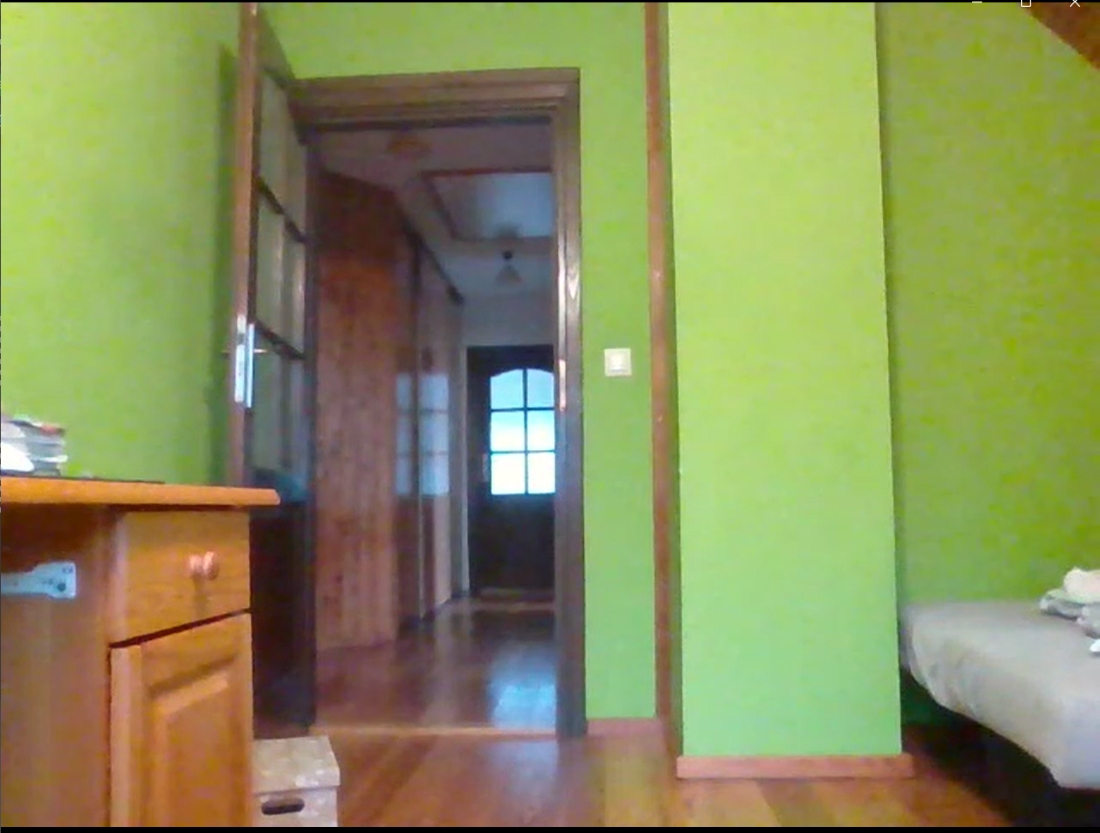
\includegraphics[width=\linewidth]{r_test_dokładności/vid_pics/1_1.jpg}
    \caption{Pomieszczenie, w którym nagrano filmy.}
    \label{fig:test-dokladnosc-scena}
\end{figure}

\begin{figure}[H]
    \centering
    \begin{minipage}{0.32\textwidth}
        \centering
        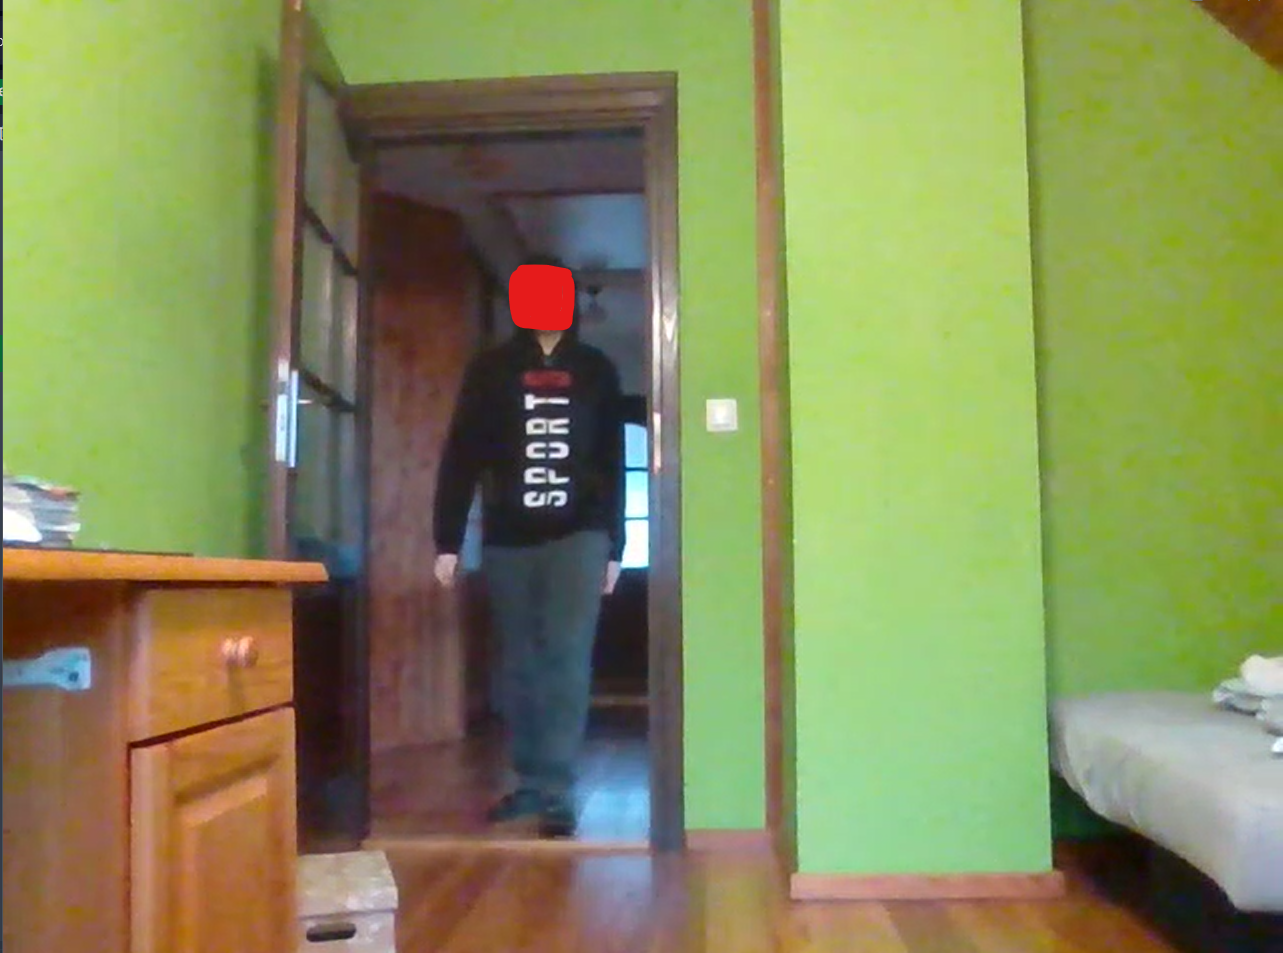
\includegraphics[width=\linewidth]{r_test_dokładności/vid_pics/1_2.png}
        \caption{Klatka filmu z człowiekiem.}
    \end{minipage}\hfill
    \begin{minipage}{0.32\textwidth}
        \centering
        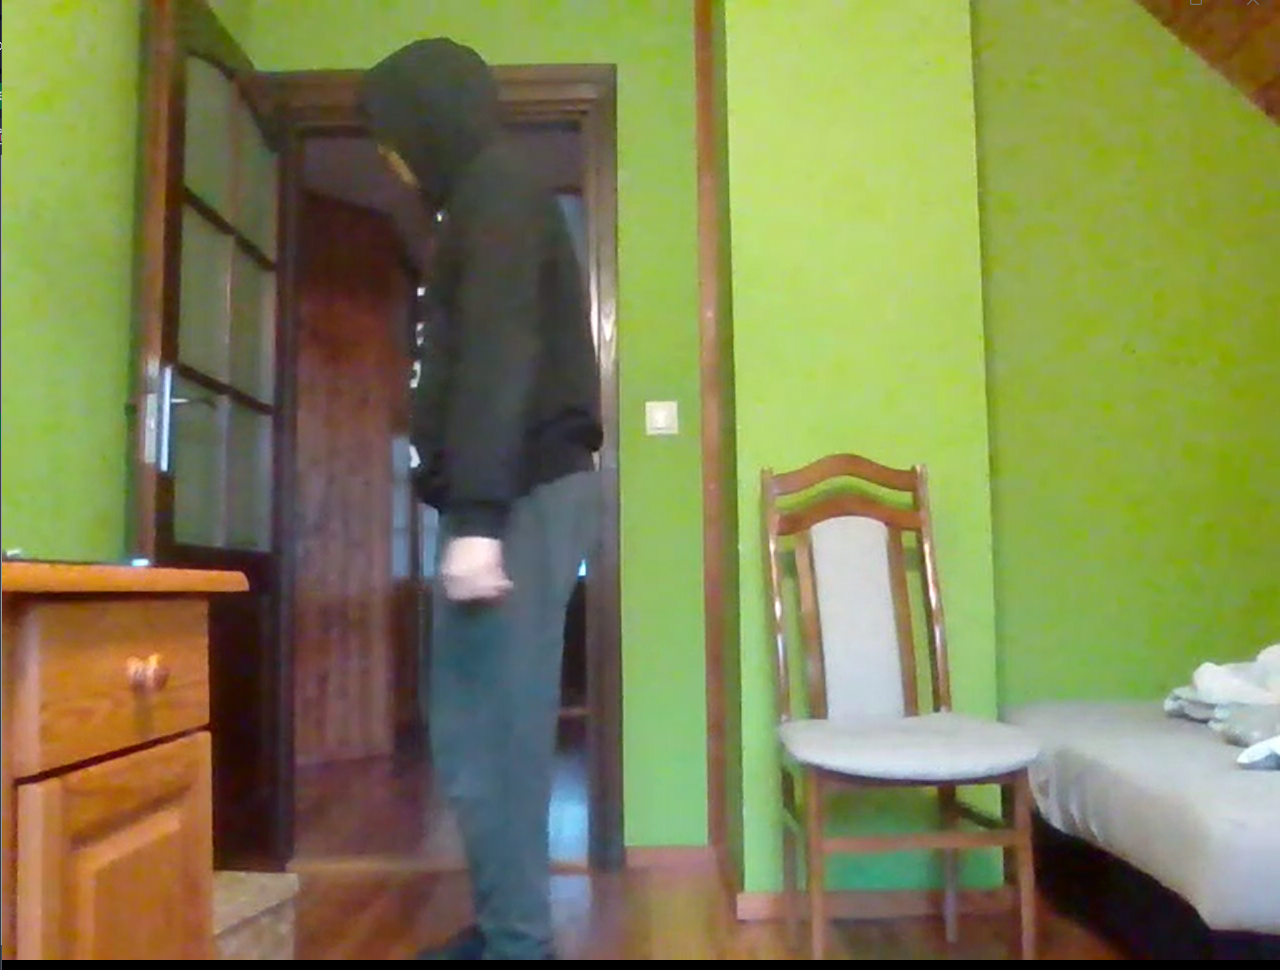
\includegraphics[width=\linewidth]{r_test_dokładności/vid_pics/1c_2.png}
        \caption{Klatka filmu z człowiekiem i krzesłem.}
    \end{minipage}\hfill
    \begin{minipage}{0.32\textwidth}
        \centering
        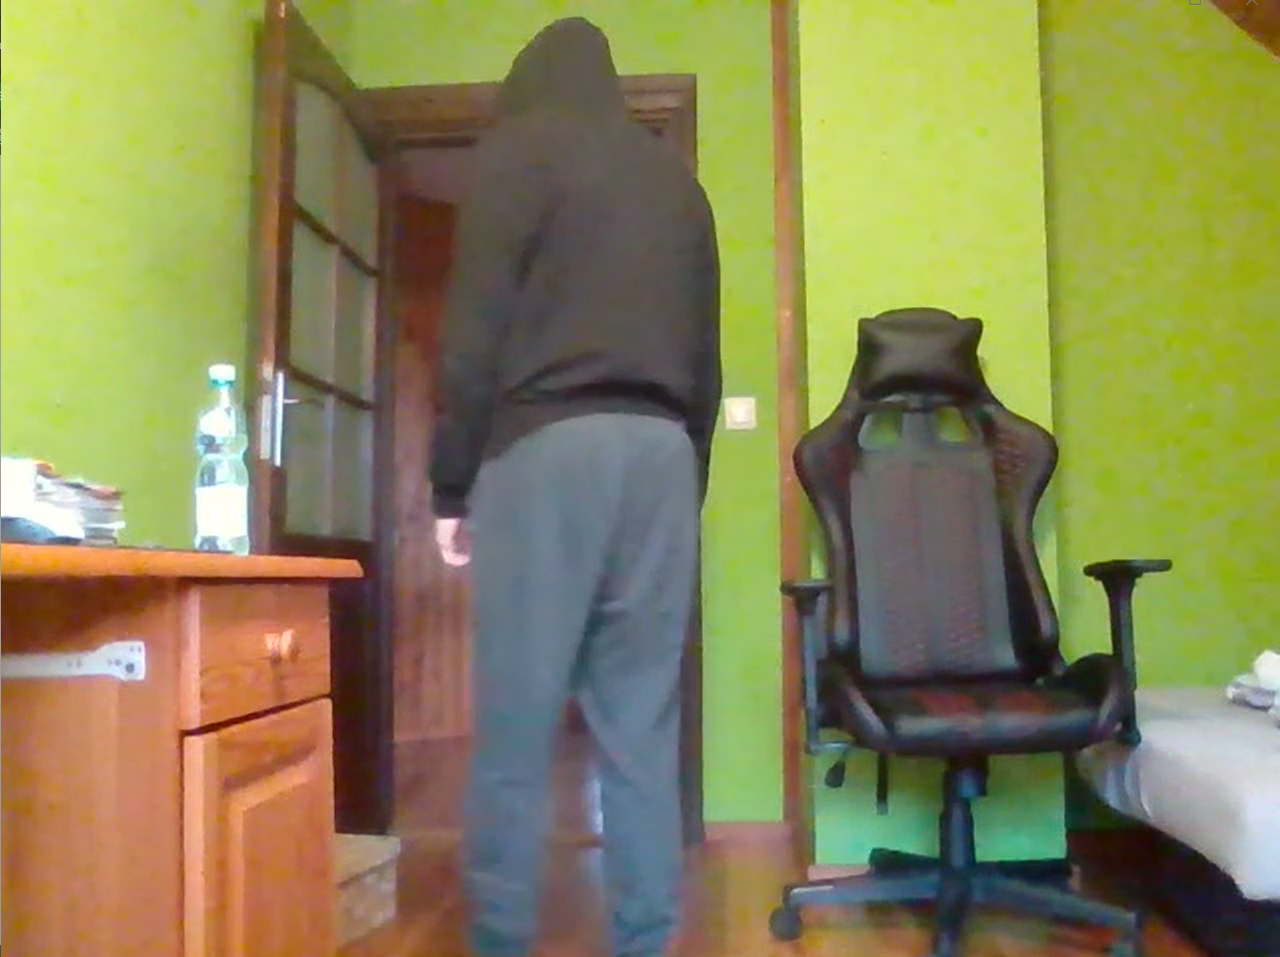
\includegraphics[width=\linewidth]{r_test_dokładności/vid_pics/1g_2.png}
        \caption{Klatka filmu z człowiekiem i fotelem.}
    \end{minipage}
    \caption{Prezentacja użytych obiektów.}
    \label{fig:all_objects}
\end{figure}
Filmy można podzielić na trzy kategorie ze względu na różne obecne w nim obiekty (wizualizacja objektów: rysunek \ref{fig:all_objects}):
\begin{itemize}
    \item człowiek
    \item człowiek, krzesło
    \item człowiek, fotel
\end{itemize}
Krzesło oraz fotel, z perspektywy filmów, są obiektami statycznymi. Przez całą długość filmu, na których występują, są umieszczone w jednej lokalizacji, a inne obiekty nie wchodzą z nimi w fizyczną interekcję.
Natomiast człowiek jest obiektem ruchomym. Jest on nieobecny przez pierwszą część każdego filmu. W drugiej części przkracza próg pomieszczenia, zbliża się do pewnego punktu widocznego w obiektywie, a pod koniec filmu wykonuje jeden pełen obrót w okół własnej osi. 

Należy podkreślić kilka istotnych kwestii dotyczących nagranych filmów:
\begin{itemize}
    \item Obecne obiekty nie wchodzą ze sobą w interakcję --- człowiek podczas ruchu nie zasłania konturów krzesła ani fotela.
    \item Generacja danych do testów nie odbywała się na każdej klatce nagranego filmu. Użyto tylko klatek, na których widoczne są pełne kontury obiektów. Pełny kontur człowieka pojawia się w momencie przekroczenia progu wejścia do pomieszczenia. W związku z powyższym, wykorzystano dwie sekcje każdego filmu: sekcję, w której człowiek był całkowicie nieobecny oraz sekcję od momentu przekroczenia progu.
\end{itemize}

Dla każdej kategorii filmu nagrano cztery warianty z różnym poziomem oświetlenia w pomieszczeniu, co daje łącznie dwanaście plików wideo do analizy. Wizualne różnice między poziomami przedstawiono na rysunku \ref{fig:person_grid} (człowiek), rysunku \ref{fig:chair_grid} (człowiek, krzesło) i rysunku \ref{fig:game_grid} (człowiek, fotel). 
Dla każdego filmu, korzystając z modelu przestrzeni barw HSV, obliczono średnią jasność oraz nasycenie. Wartości te zaprezentowano w tabeli \ref{tab:saturation-value-table}. Obliczenia polegały na wyznaczeniu średniej wartości jasności i nasycenia dla każdej klatki obrazu na podstawie wszystkich pikseli. Następnie wyznaczono średnią z uzyskanych wartości dla wszystkich klatek w filmie.
\begin{table}[H]
    \centering
    \caption{Jasność i nasycenie dla każdego nagranego filmu.}
    \begin{tabular}{|c|c|c|c|}
    \hline
    Nr sceny:          & Obecne obiekty    & Jasność & Nasycenie \\ \hline
    \multirow{3}{*}{1} & człowiek          & 152.73  & 107.3     \\ \cline{2-4} 
                       & człowiek, krzesło & 149.92  & 119.07    \\ \cline{2-4} 
                       & człowiek, fotel   & 152.68  & 111.47    \\ \hline
    \multirow{3}{*}{2} & człowiek          & 134.64  & 93.48     \\ \cline{2-4} 
                       & człowiek, krzesło & 139.14  & 90.71     \\ \cline{2-4} 
                       & człowiek, fotel   & 133.77  & 83.29     \\ \hline
    \multirow{3}{*}{3} & człowiek          & 41.59   & 123.48    \\ \cline{2-4} 
                       & człowiek, krzesło & 38.91   & 132.31    \\ \cline{2-4} 
                       & człowiek, fotel   & 38.12   & 124.31    \\ \hline
    \multirow{3}{*}{4} & człowiek          & 25.47   & 90.92     \\ \cline{2-4} 
                       & człowiek, krzesło & 25.3    & 100.8     \\ \cline{2-4} 
                       & człowiek, fotel   & 24.88   & 108.5     \\ \hline
    \end{tabular}
    \label{tab:saturation-value-table}
    \end{table}
\begin{figure}[H]
    \centering
    \begin{minipage}{0.45\textwidth}
        \centering
        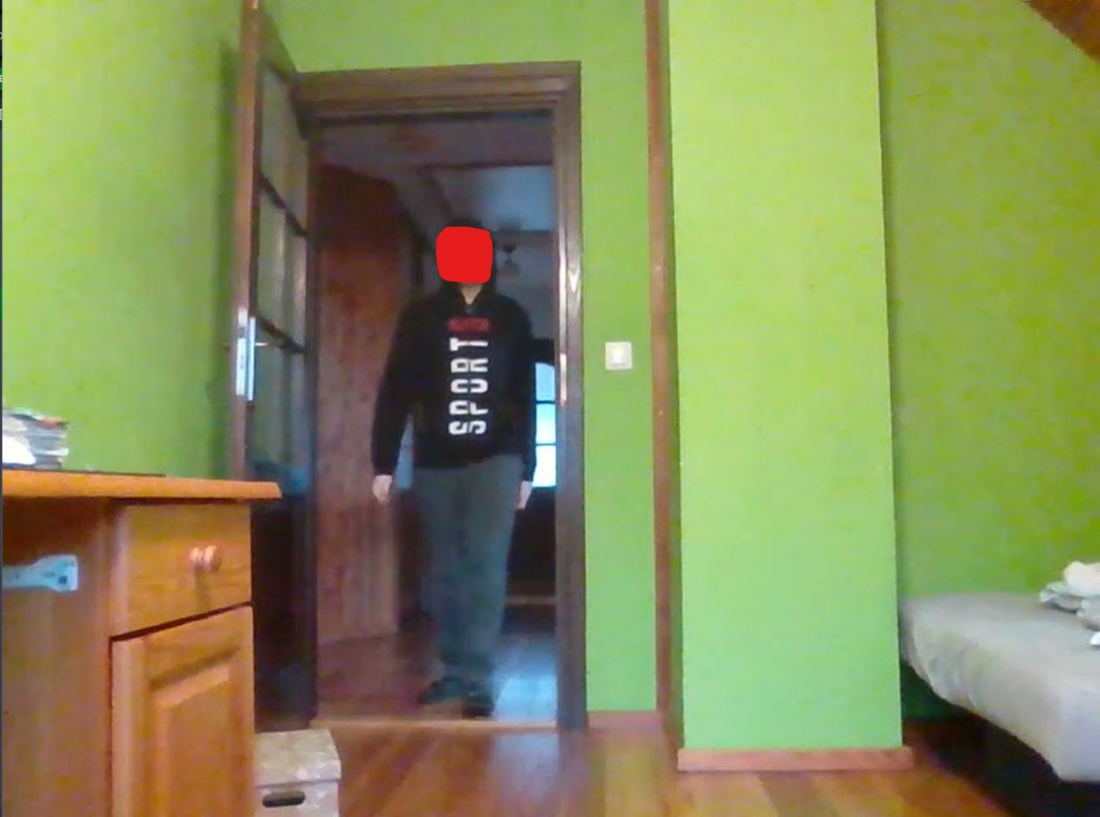
\includegraphics[width=\linewidth]{r_test_dokładności/vid_pics/1_2.jpg}
    \end{minipage}\hfill
    \begin{minipage}{0.45\textwidth}
        \centering
        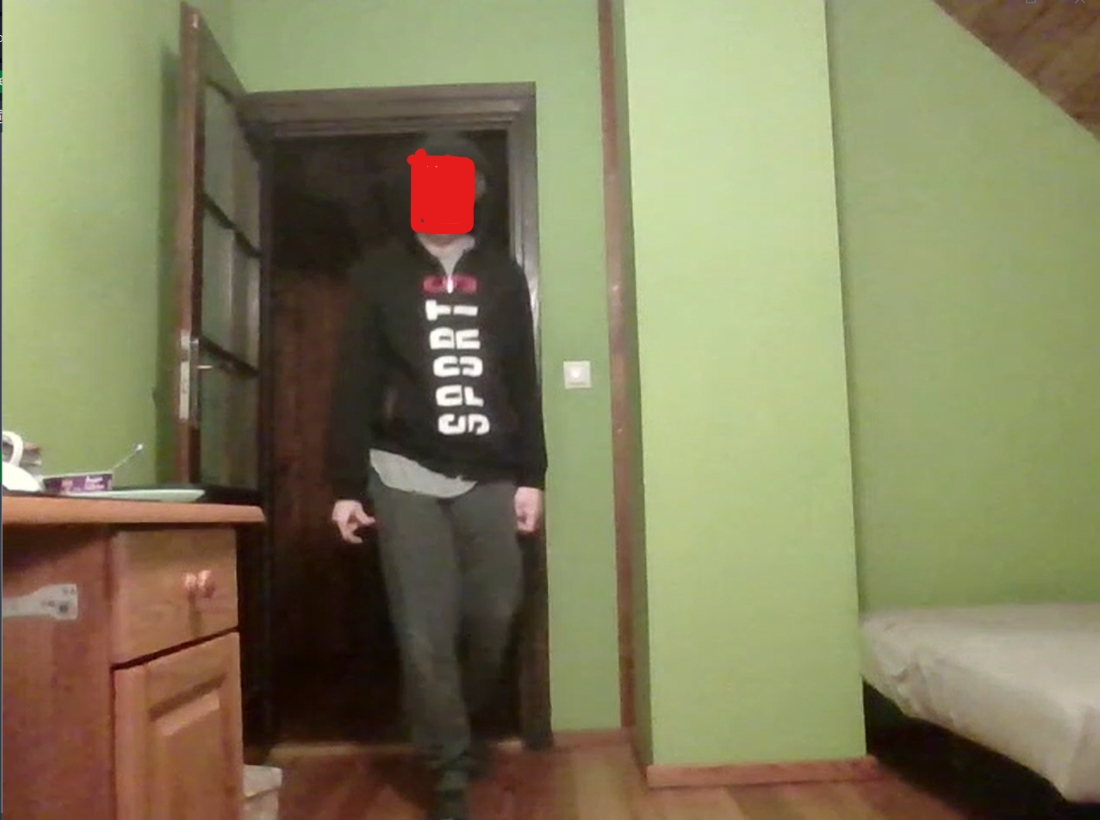
\includegraphics[width=\linewidth]{r_test_dokładności/vid_pics/2_2.jpg}
    \end{minipage}
    \vskip\baselineskip
    \begin{minipage}{0.45\textwidth}
        \centering
        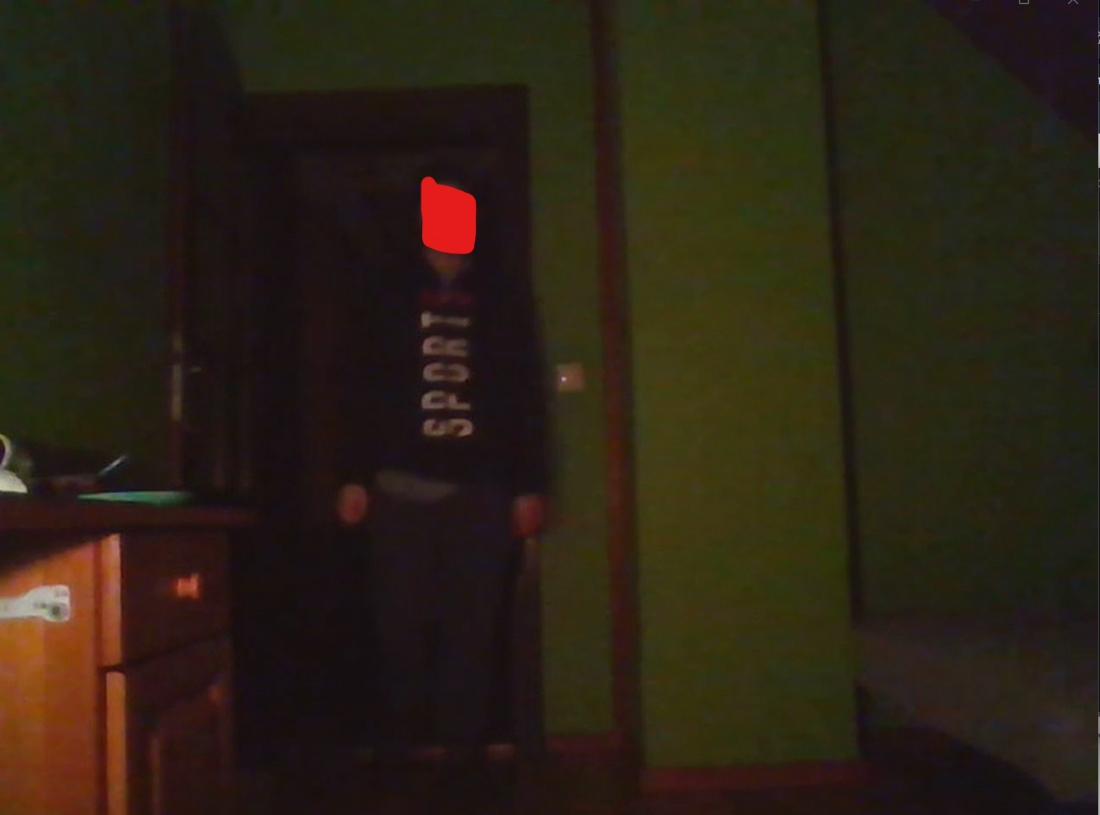
\includegraphics[width=\linewidth]{r_test_dokładności/vid_pics/3_2.jpg}
    \end{minipage}\hfill
    \begin{minipage}{0.45\textwidth}
        \centering
        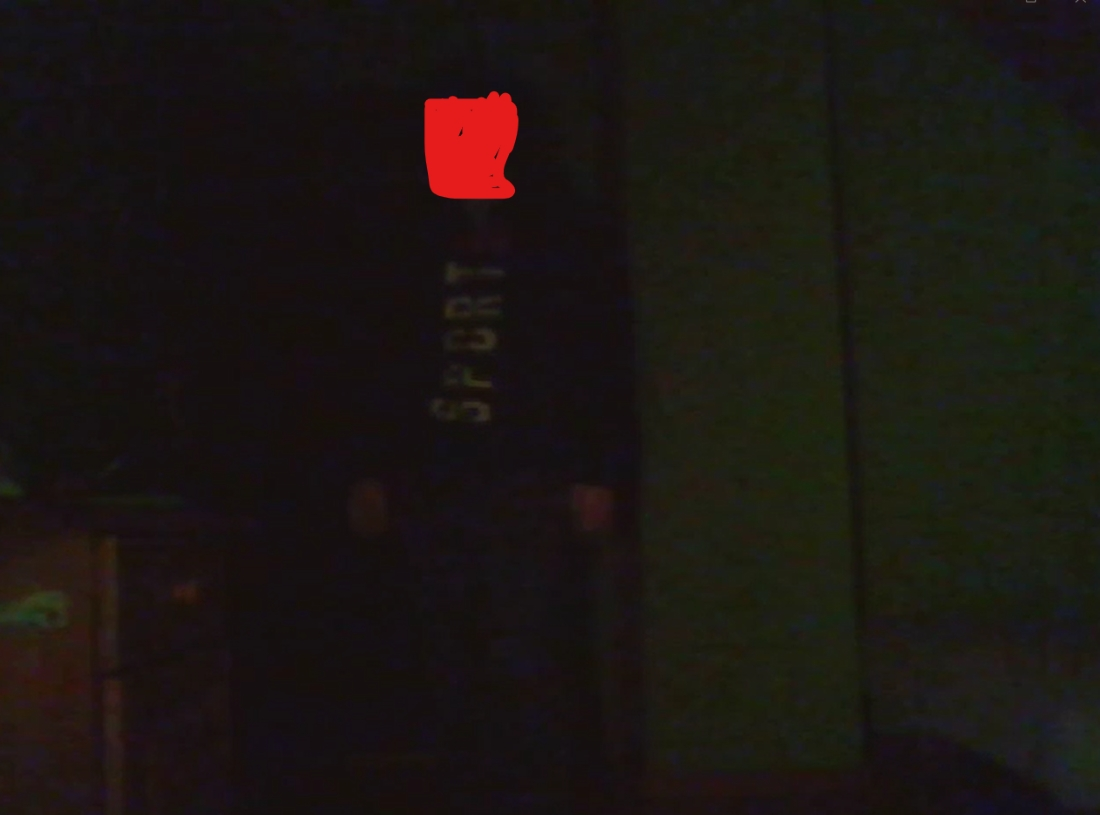
\includegraphics[width=\linewidth]{r_test_dokładności/vid_pics/4_2.jpg}
    \end{minipage}
    \caption{Poziomy oświetlenia dla filmów z obecnym człowiekiem}
    \label{fig:person_grid}
\end{figure}
\begin{figure}[H]
    \centering
    \begin{minipage}{0.45\textwidth}
        \centering
        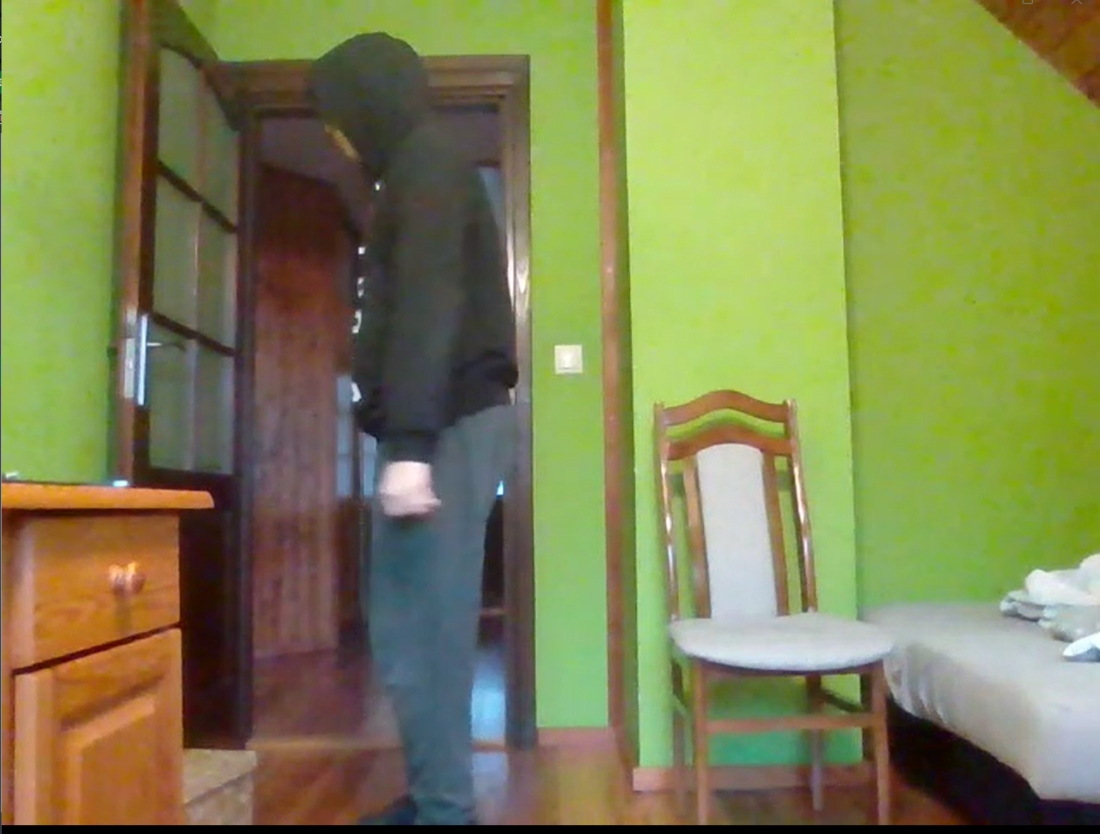
\includegraphics[width=\linewidth]{r_test_dokładności/vid_pics/1c_2.jpg}
    \end{minipage}\hfill
    \begin{minipage}{0.45\textwidth}
        \centering
        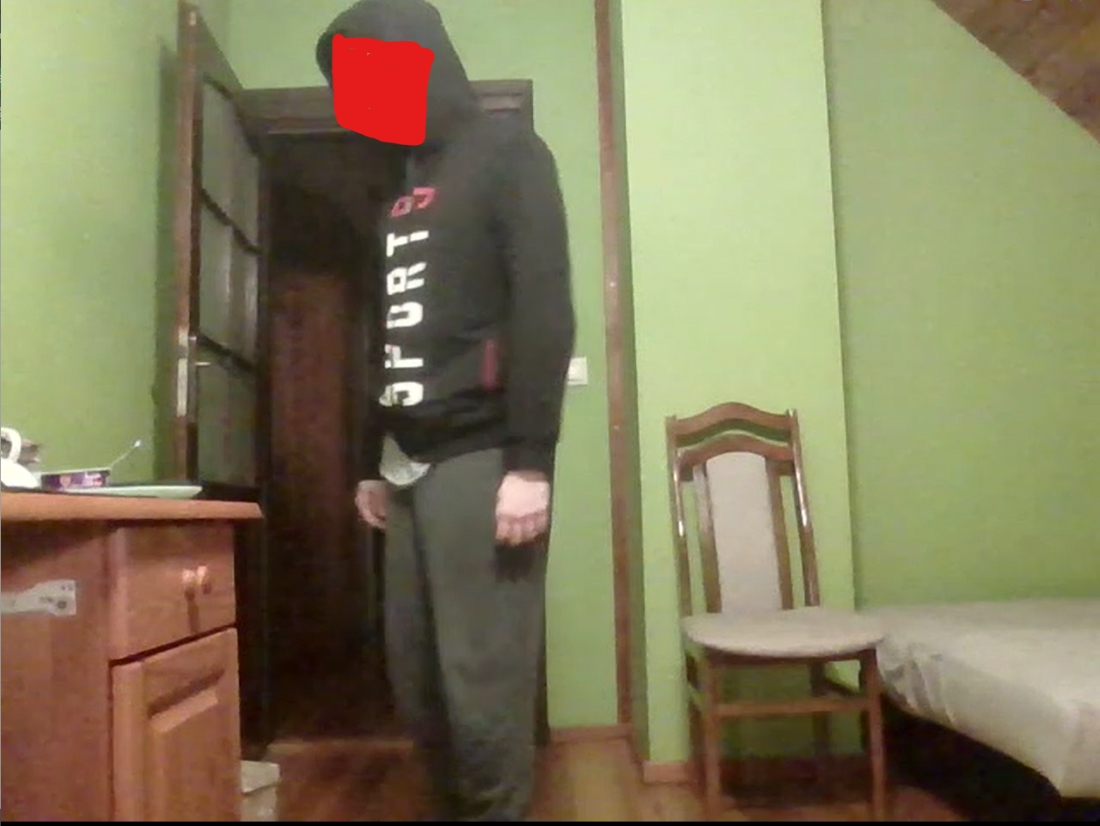
\includegraphics[width=\linewidth]{r_test_dokładności/vid_pics/2c_2.jpg}
    \end{minipage}
    \vskip\baselineskip
    \begin{minipage}{0.45\textwidth}
        \centering
        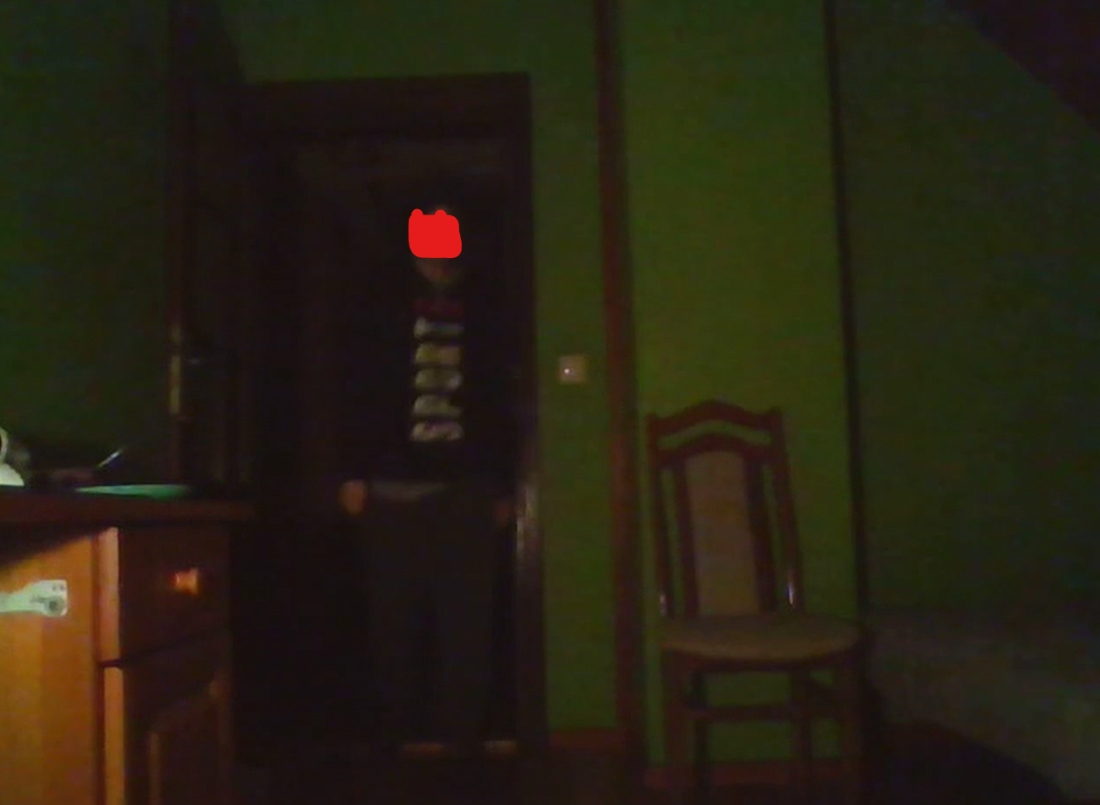
\includegraphics[width=\linewidth]{r_test_dokładności/vid_pics/3c_2.jpg}
    \end{minipage}\hfill
    \begin{minipage}{0.45\textwidth}
        \centering
        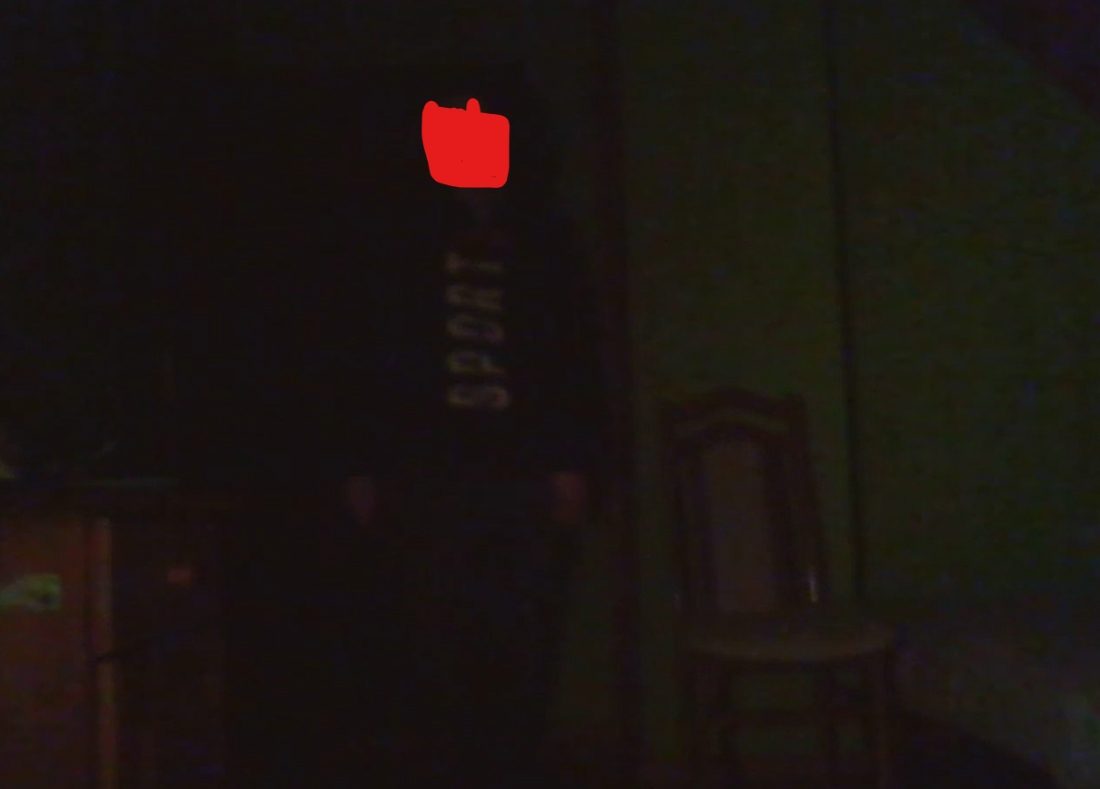
\includegraphics[width=\linewidth]{r_test_dokładności/vid_pics/4c_2.jpg}
    \end{minipage}
    \caption{Poziomy oświetlenia dla filmów z obecnym człowiekiem i krzesłem}
    \label{fig:chair_grid}
\end{figure}
\begin{figure}[H]
    \centering
    \begin{minipage}{0.45\textwidth}
        \centering
        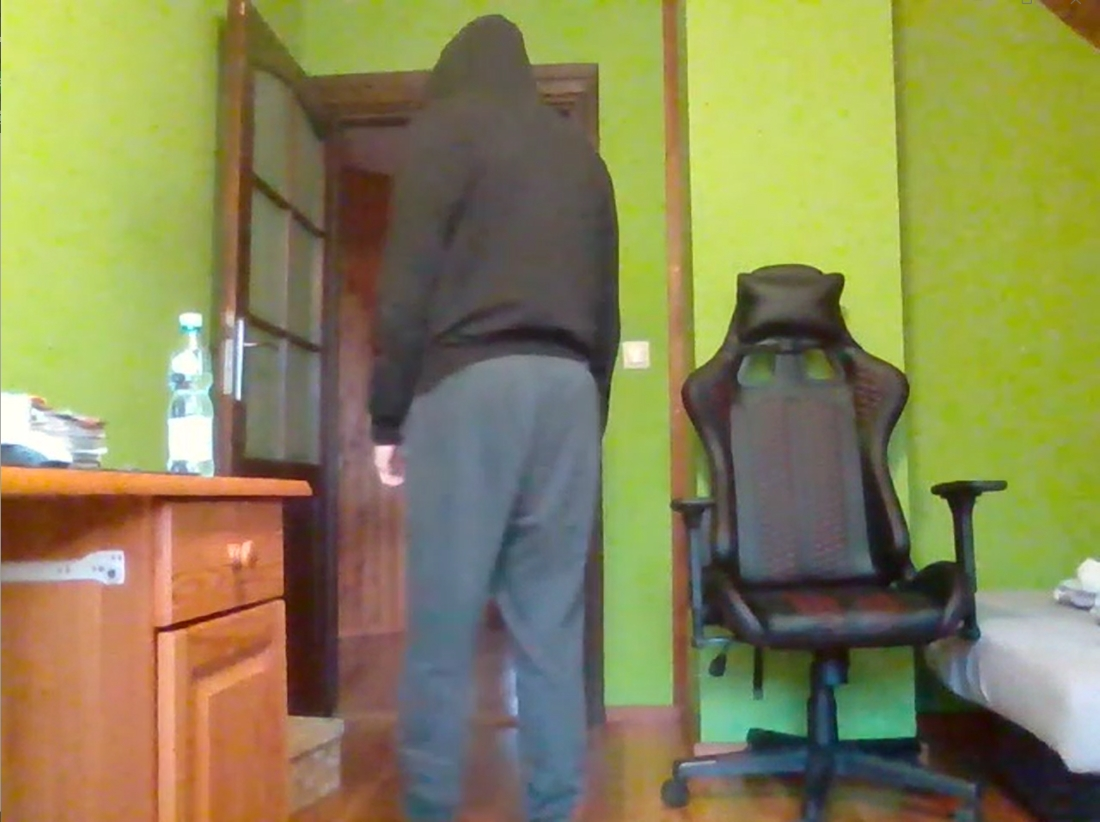
\includegraphics[width=\linewidth]{r_test_dokładności/vid_pics/1g_2.jpg}
    \end{minipage}\hfill
    \begin{minipage}{0.45\textwidth}
        \centering
        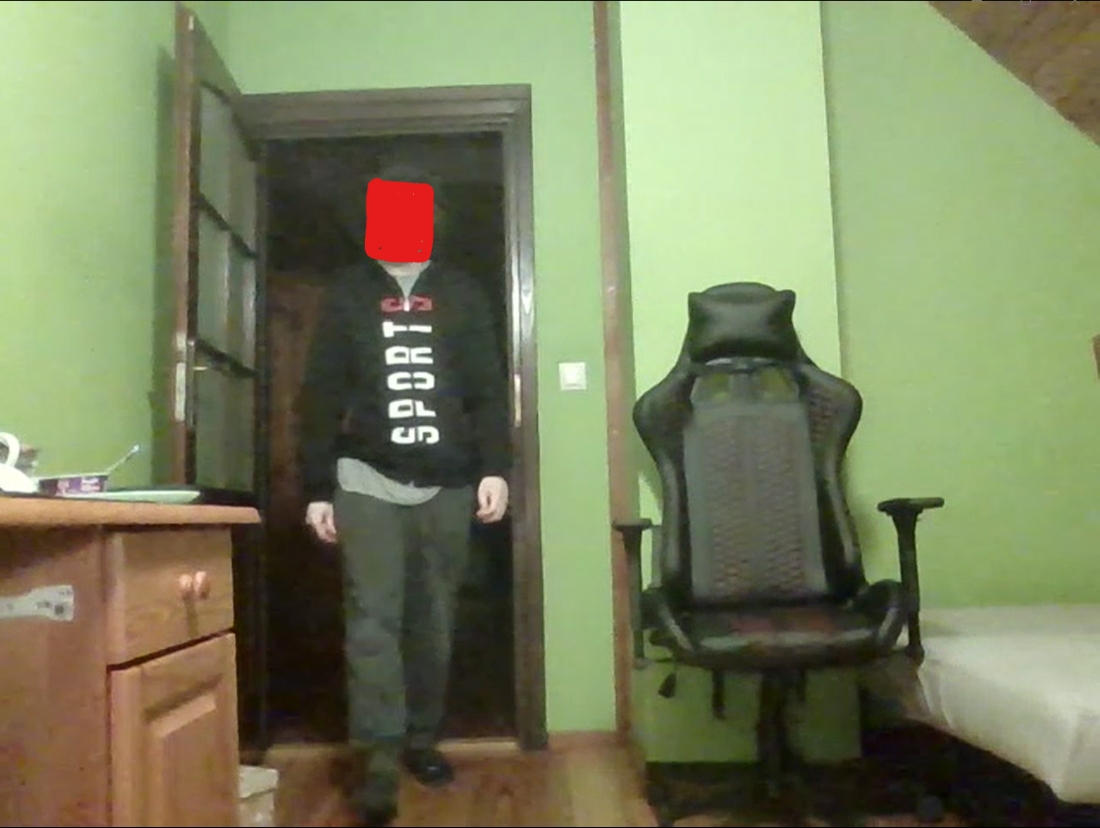
\includegraphics[width=\linewidth]{r_test_dokładności/vid_pics/2g_2.jpg}
    \end{minipage}
    \vskip\baselineskip
    \begin{minipage}{0.45\textwidth}
        \centering
        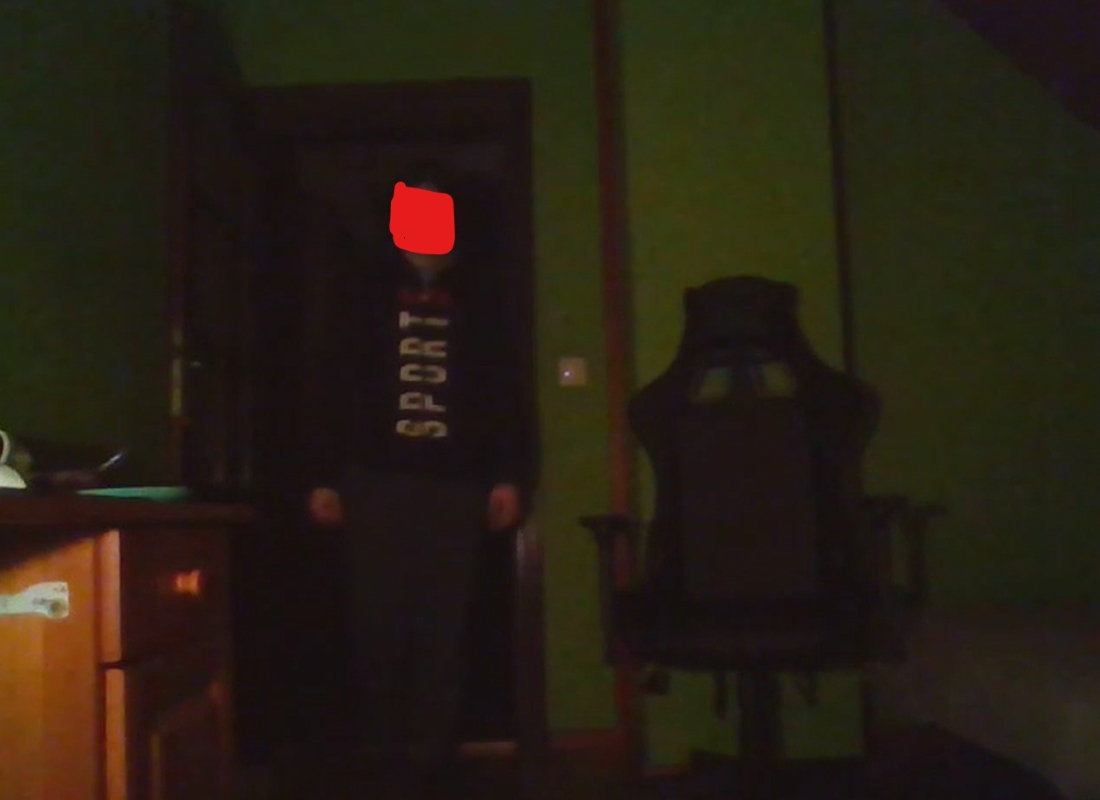
\includegraphics[width=\linewidth]{r_test_dokładności/vid_pics/3g_2.jpg}
    \end{minipage}\hfill
    \begin{minipage}{0.45\textwidth}
        \centering
        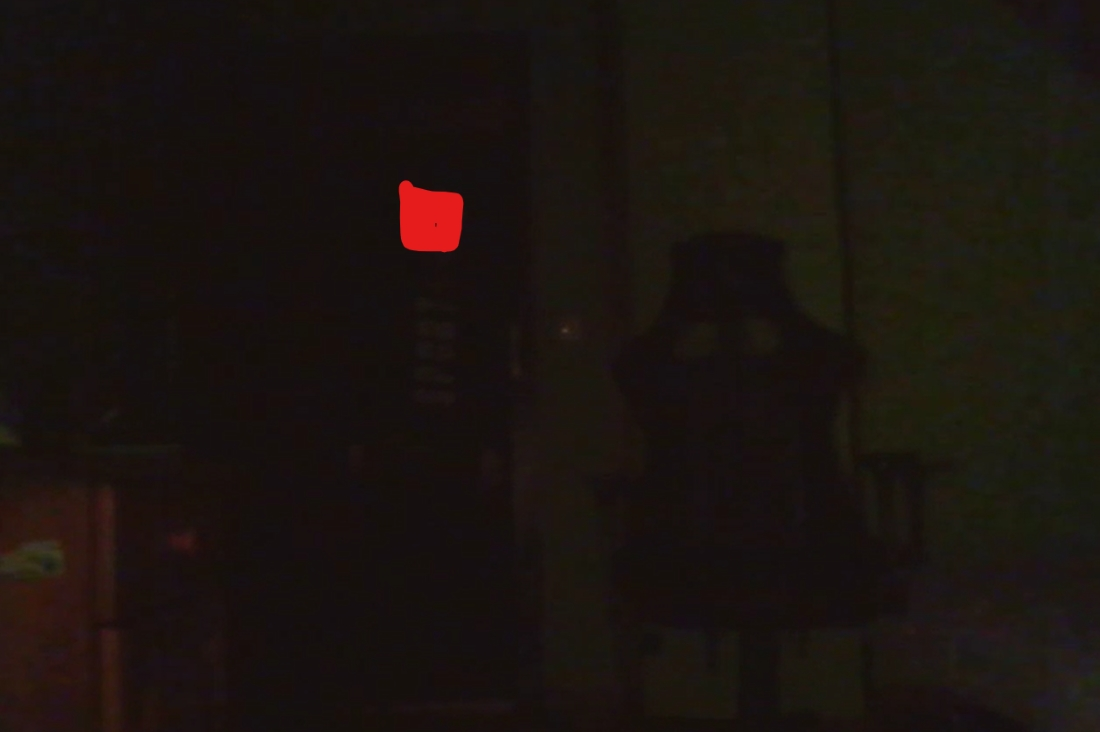
\includegraphics[width=\linewidth]{r_test_dokładności/vid_pics/4g_2.jpg}
    \end{minipage}
    \caption{Poziomy oświetlenia dla filmów z obecnym człowiekiem i fotelem}
    \label{fig:game_grid}
\end{figure}







\subsection{Metryki i dane wynikowe używane w testach}
Na podstawie opisanych dwunastu plików wideo wygenerowano dane do analizy w testach dla każdego z nich. Dane te to podstawowe metryki używane w klasyfikacji binarnej. Są to: wynik prawdziwy pozytywny (TP), wynik prawdziwy negatywny (TN), wynik fałszywy pozytywny (FP), wynik fałszywy negatywny (FN). 
Zaprojektowane testy sprawdzają tylko jedną klasę na test --- np. dla ewaluacji klasyfikacji klasy \emph{człowiek}, ignorowane są wykrycia innych klas. Co więcej, w niniejszym systemie nacisk kładziony jest na alarmowanie użytkownika o obecności obiektu, dlatego też uznano, iż więcej niż jedna detekcja klasy będzie przypisana do tej samej metryki co detekcja pojedynczego obiektu. 

Biorąc to pod uwagę, definicję metryk skonstruowano następująco: \\ \\ \noindent
Znaczenie skrótów z tabeli \ref{tab:saturation-value-table}: \\
$\emptyset$ -- brak wystąpienia obiektu wykrywanej klasy \\
x -- pojedyńcze wystąpienie obiektu wykrywanej klasy \\
n*x -- wielokrotne wystąpienie obiektu wykrywanej klasy
\begin{table}[H]
    \centering
    \caption{Definicja metryk generowanych podczas testów detekcji obiektów.}
    \begin{tabular}{|>{\centering\arraybackslash}m{2cm}|>{\centering\arraybackslash}m{2cm}|>{\centering\arraybackslash}m{2.5cm}|>{\raggedright\arraybackslash}m{7.5cm}|}
    \hline
    Metryka & Obiekty na nagraniu & Obiekty wykryte przez detektor & \multicolumn{1}{c|}{Opis} \\ \hline



    \multirow{2}{*}{TP} & \multirow{2}{*}{x} & x & \multirow{2}{7.5cm}{Detektor wykrył jeden lub więcej obiektów klasy x, gdy obiekt x był obecny.} \\ \cline{3-3}

     &  & n*x & \\ \cline{1-4}



    TN & $\emptyset$ & $\emptyset$ & Detektor nie wykrył ani jednego obiektu klasy x, gdy obiekt x był nieobecny. \\ \hline

    

    \multirow{2}{*}{TN} & \multirow{2}{*}{$\emptyset$} & x & \multirow{2}{7.5cm}{Detektor wykrył jeden lub więcej obiektów klasy x, mimo że obiekt był nieobecny.} \\ \cline{3-3}

     &  & n*x & \\ \cline{1-4}



    FN & x & $\emptyset$ & Detektor nie wykrył ani jednego obiektu klasy x, mimo że obiekt był obecny. \\ \hline
    \end{tabular}
\end{table}

Generacja metryk wynikowych odbywa się w następująco:
\begin{enumerate}
    \item Wybierany jest film.
    \item Dla filmu metryki generowane są dla każdej badanej wartości progu ufności.
    \item Dla progu ufności analizowana jest każda klatka spełniająca wymagania opisane w rozdziale \ref{sec:zrodlo_wideo}. Dana klatka jest kategoryzowana do jednej z metryk.
    \item Metryka wynikowa to liczba klatek przypisanych do tej metryki.
\end{enumerate} 
Przykład wygenerowanych wyników prezentuje tabela \ref{tab:example-generated}.
\begin{table}[H]
    \centering
    \caption{Struktura wygenerowanych wyników na przykładzie częściowych wyników dla filmu z obecnym człowiekiem dla poziomu oświetlania nr 1. Wartości metryk to liczba klatek filmu przypisana do każdej z nich.}
    \begin{tabular}{ccccc}
    \hline
    \multicolumn{1}{|c|}{Próg   ufności} & \multicolumn{1}{c|}{TP}                    & \multicolumn{1}{c|}{TN}                    & \multicolumn{1}{c|}{FP}                    & \multicolumn{1}{c|}{FN}                    \\ \hline
    \multicolumn{1}{|c|}{0}                                 & \multicolumn{1}{c|}{100}                   & \multicolumn{1}{c|}{0}                     & \multicolumn{1}{c|}{122}                   & \multicolumn{1}{c|}{0}                     \\ \hline
    \multicolumn{1}{|c|}{0.01}                              & \multicolumn{1}{c|}{100}                   & \multicolumn{1}{c|}{49}                    & \multicolumn{1}{c|}{73}                    & \multicolumn{1}{c|}{0}                     \\ \hline
    \multicolumn{1}{|c|}{0.02}                              & \multicolumn{1}{c|}{100}                   & \multicolumn{1}{c|}{104}                   & \multicolumn{1}{c|}{18}                    & \multicolumn{1}{c|}{0}                     \\ \hline
    \multicolumn{1}{|c|}{0.03}                              & \multicolumn{1}{c|}{100}                   & \multicolumn{1}{c|}{120}                   & \multicolumn{1}{c|}{2}                     & \multicolumn{1}{c|}{0}                     \\ \hline
    \multicolumn{1}{|c|}{0.04}                              & \multicolumn{1}{c|}{100}                   & \multicolumn{1}{c|}{122}                   & \multicolumn{1}{c|}{0}                     & \multicolumn{1}{c|}{0}                     \\ \hline
    \multicolumn{5}{c}{$\bullet$ $\bullet$   $\bullet$ $\bullet$ $\bullet$ $\bullet$ $\bullet$ $\bullet$ $\bullet$   $\bullet$ $\bullet$ $\bullet$ $\bullet$ $\bullet$ $\bullet$ $\bullet$   $\bullet$ $\bullet$ $\bullet$ $\bullet$ $\bullet$} \\ \hline
    \multicolumn{1}{|c|}{0.96}                              & \multicolumn{1}{c|}{0}                     & \multicolumn{1}{c|}{122}                   & \multicolumn{1}{c|}{0}                     & \multicolumn{1}{c|}{100}                   \\ \hline
    \multicolumn{1}{|c|}{0.97}                              & \multicolumn{1}{c|}{0}                     & \multicolumn{1}{c|}{122}                   & \multicolumn{1}{c|}{0}                     & \multicolumn{1}{c|}{100}                   \\ \hline
    \multicolumn{1}{|c|}{0.98}                              & \multicolumn{1}{c|}{0}                     & \multicolumn{1}{c|}{122}                   & \multicolumn{1}{c|}{0}                     & \multicolumn{1}{c|}{100}                   \\ \hline
    \multicolumn{1}{|c|}{0.99}                              & \multicolumn{1}{c|}{0}                     & \multicolumn{1}{c|}{122}                   & \multicolumn{1}{c|}{0}                     & \multicolumn{1}{c|}{100}                   \\ \hline
    \multicolumn{1}{|c|}{1}                                 & \multicolumn{1}{c|}{0}                     & \multicolumn{1}{c|}{122}                   & \multicolumn{1}{c|}{0}                     & \multicolumn{1}{c|}{100}                   \\ \hline
    \end{tabular}
    \label{tab:example-generated}
    \end{table}
